\section{Projektmål}
Applikationen är ett verktyg för att tydligt få en överblick över händelser och flöden i CI-processer för ett system, exempelvis byggen och tester. Applikationens målgrupp är företag som bedriver mjukvaruutveckling med större utvecklingsteam. Företaget använder sig i dagsläget av CI och vill kunna upptäcka flaskhalsar och förbättra sitt arbetsflöde. Applikationen är en webbaserad tjänst som kommer att skrivas i JavaScript. Data som visualiseras i applikationen kommer från valfritt CI-system, och generaliseras med hjälp av ramverket Eiffel. Händelser och flöden visualiseras genom interaktiva grafer där användaren kan välja att visa data i flera olika nivåer för att kunna dra slutsatser sitt utvecklingsflöde. 
\\
För mer detaljerad information se kravspecificationen.

\iffalse
\begin{figure}[h]
    \centering
    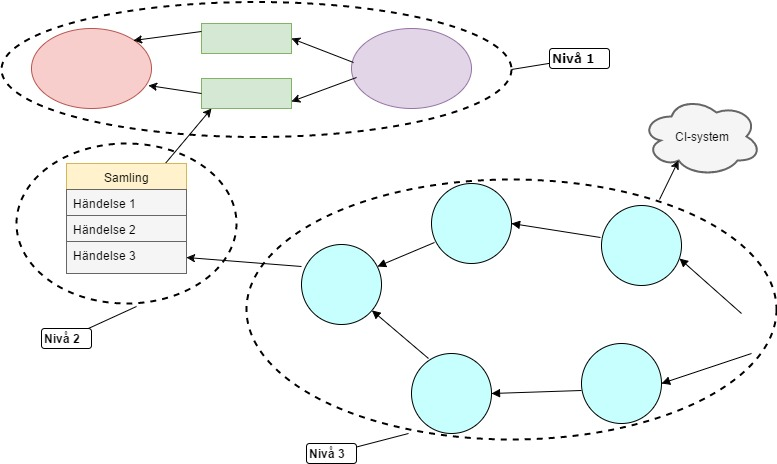
\includegraphics[width=\textwidth]{Visualization}
    \caption{De olika nivåerna av systemet, godtyckligt färgade.}
    \label{fig:system_overview}
\end{figure}
\fi

\subsection{Affärsmål}
Applikationen ska visualisera händelser i ett CI-system så att en beslutsfattande person som inte har kunskaper inom programmering ska kunna fatta beslut hur resurser ska fördelas.

\subsection{Systemmål}
För systemmål se arkitekturdokumentet.

\subsection{Kvalitetsmål}
För kvalitetsmål se kvalitetplanen.
